\subsection{Optimization using a surrogate model}\label{model-based}
In cases where evaluating the objective function at a specific point is time-consuming or computationally expensive, it can be useful to employ a surrogate model for the objective function during optimization. We define a surrogate model of the given problem as the problem

\begin{equation}
	\min_{\vec{x} \in \mathbf{\tilde{X}}} \tilde{f}(\vec{x}),
\end{equation}
where
\begin{equation}
	\mathbf{\tilde{X}} = \left\{ \vec{x} \in \mathbf{D} \subseteq \mathbb{R}^n \ \middle| \ \vec{\tilde{g}} (\vec{x}) \leq \vec{0} \wedge \vec{\tilde{h}} (\vec{x}) = \vec{0} \right\},
\end{equation}
and the functions \( \tilde{f}, \vec{\tilde{g}} \), and \( \vec{\tilde{h}} \) have characteristics similar to those of the functions \( f, \vec{g} \), and \( \vec{h} \) in the original problem. The characteristics of \( \tilde{f}, \vec{\tilde{g}} \), and \( \vec{\tilde{h}} \) are intentionally left undefined, reflecting the fact that the surrogate model does not necessarily need to be an accurate approximation of the original problem \cite{BBO-textbook, two-decades, Kramer2011}. A good approximative model may not always be a suitable surrogate for optimization purposes, a situation illustrated in Figure \ref{fig:surrogate}.

\begin{figure}[H]
	\centering
	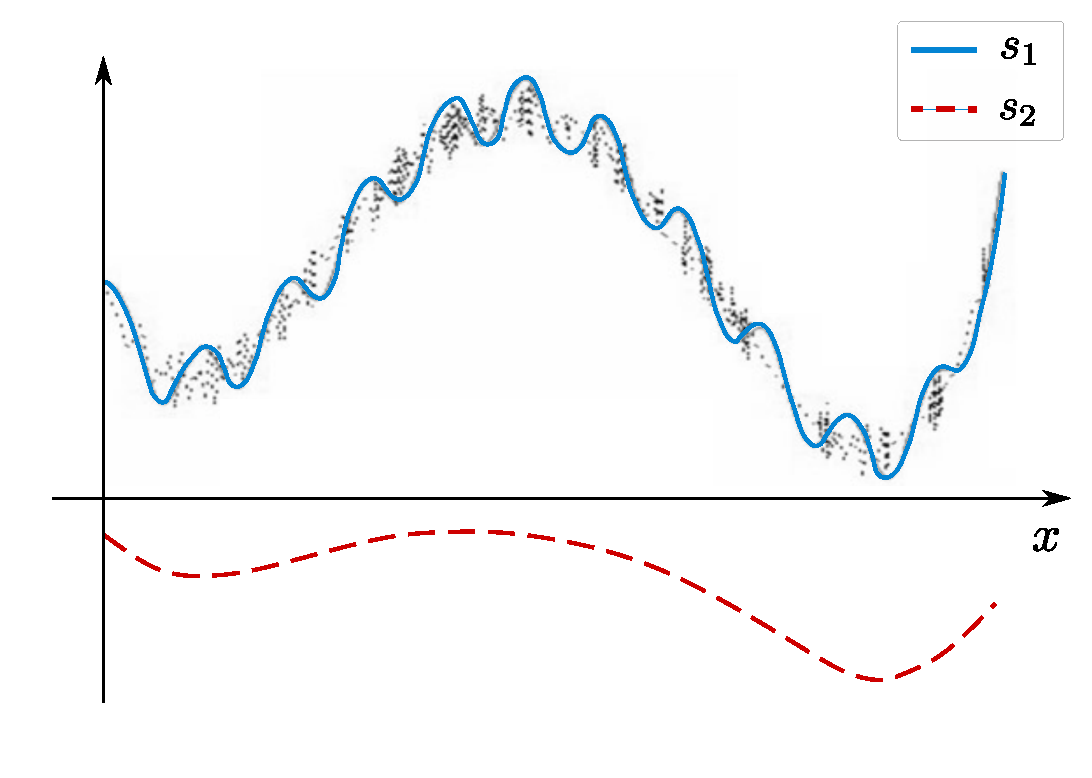
\includegraphics[width=0.6\textwidth]{figures/surrogate.pdf}
	\caption{An illustration of two surrogate models, $ s_1 $ and $ s_2 $. The black points represent noisy values of the objective function. While using surrogate model $ s_1 $ represents a better choice for approximating the function, it is not suitable for optimization since $ s_1 $ contains many undesirable stationary points that the original objective function does not have. On the other hand, while surrogate model $ s_2 $ is not as accurate in approximating the function's values, it is a better choice for optimization because the stationary points of $ s_2 $ are almost identical to those of the optimized objective function.}
	\label{fig:surrogate}
\end{figure}

Using a surrogate model in optimization is often just a part of a more complex optimization method. Surrogate models can, for example, be used within GPS and MADS methods described in Section~\ref{direct-search}, where, during the poll step, we first evaluate the surrogate function \( \tilde{f} \) at the points from the poll set, sort these values, and use them to sort the poll set used to evaluate the original function \( f \). This potentially allows us to significantly reduce the time required to complete the poll step, as sorting the points increases the probability of finding a better estimate of the solution at one of the first examined points \cite{BBO-textbook}. Surrogate models can also be used within other methods to accelerate the optimization process, and their application is discussed in detail in \cite{BBO-textbook, two-decades}.
